%\subsection{Experiment}
%\label{sec:experiment}

\newcommand{\takeaway}[1]{
\vspace{6pt}
\noindent\fbox{\parbox{\textwidth}{#1}}
\vspace{6pt}
}
\subsection{Experimental Setup}
 In this study, we designed an experiment from
 the same benchmark suite used for evaluation of the \ucalg ~and \ucbfalg ~algorithms in \cite{Ghass16}.
 The benchmark contains 476 Lustre models
 from~\cite{Hagen08:FMCAD} and \cite{QFCS15:backes,hilt2013}.
 Most of
the benchmark models from~\cite{Hagen08:FMCAD} are small (10kB or less,
with 6-40 equations) and include a range of hardware benchmarks and
software problems involving counters.
However, models from \cite{QFCS15:backes,hilt2013} are industrial cases with over 600 equations around 80kB.
Each benchmark model has a single property to analyze.
For each test model, we computed \aivcalg , \ucalg , and \ucbfalg ~algorithms
in a configuration with
the \texttt{Z3} solver and the fastest mode of \texttt{JKind} (running K-induction and PDR in parallel). The experiments
were run on an  Intel(R) i5-4690, 3.50GHz,
16 GB memory machine.
%\footnote{\noindent ~The benchmarks, all raw experimental results,
%  and computed data are available on \cite{expr}.}

We would like to evaluate the efficiency
 of our algorithms and compare it with the \ucalg ~and \ucbfalg ~algorithms.
 Efficiency is computed in terms of wall-clock time. Therefore, we investigate the following research questions:
\begin{itemize}
  \item \textbf{RQ1)} How does the \aivcalg ~algorithm perform compared to the \ucalg ~and \ucbfalg ~algorithms?
  \item \textbf{RQ2)} How is the \aivcalg ~algorithm affected by the number of IVCs (diversity) and verification time (time a property takes to be proved)?
%
%  \item \textbf{RQ3)} How does approximating minimality influence the performance of the \aivcalg ~algorithm?
%  In other words, we would like to determine, for the implementation of the \getivc ~procedure, whether it would be better to use \ucalg ~or \ucbfalg .
%  \item \textbf{RQ4)} How did the pre-set timeout manifest itself in the experimental results?
\end{itemize}


\subsection{Experimental Results}

\section{Results}
\label{sec:results}

\newcommand{\takeaway}[1]{
\vspace{6pt}
\noindent\fbox{\parbox{\columnwidth}{#1}}
\vspace{6pt}
}

In this section, we examine our experimental results from three perspectives: performance, minimality of \ucalg results and diversity.

\iffalse
\mike{Results and Discussion:}
\begin{itemize}
    \item (Overview) Give an overview of results, possibly referencing a graph or two.
    \item Statistical analysis: provide positive and null hypotheses for the research questions.
    \item Evaluation of research questions: statistical results and explanations of the graphs.  One subsection per research question?
    \item Threats to validity: what are our threats?
    Internal validity: not really necessary, I think.
    External validity (how much can the results be generalized):
        1. currently all models are *very small*;
        2. Many programs were drawn from mutations of a relatively small number of ``seed'' programs;
        3. The models are written in Lustre rather than FOL.  This means that the
            top-level conjunctions are all over equations rather than general
            form;
        4. Others?!?
    Construct validity: we are measuring what we think we're measuring: IVC and minimality are reasonably defined.  For discussions of ``completeness'' and ``traceability'' we need to be clear about any claims (probably not in this paper).
\end{itemize}
\fi

\subsection{Performance}
\label{sec:performance}

In this subsection, we examine the performance of our inductive validity core algorithms (research question \textbf{RQ1}).  First we examine the performance overhead of the \ucalg algorithm over the time necessary to find a proof using inductive model checking.  To examine this question, we use the default {\em fastest} option of JKind which terminates when either the k-induction or PDR algorithm finds a proof.  To measure the performance overhead of the \ucalg algorithm, we execute it over the proof generated by the {\em fastest} option.

Since the \ucalg algorithm uses the UNSAT-core facilities of the underlying SMT solver, the performance is dependent on the efficiency of this part of the solver.  Examining Tables~\ref{tab:runtime-ucalg} and~\ref{tab:overhead-ucalg}, it is possible to examine both the aggregate computation time for analysis using the four solvers under evaluation and the overhead imposed by the \ucalg algorithm.  The data suggests that yices (the default solver in JKind) and z3 are the most performant solvers both in terms of computation time and overhead.  Figure~\ref{fig:runtimeall} allows a visualization of the overhead for the \ucalg algorithm running different tools (as well as the \bfalg, discussed below).  For this figure, models are ranked on the x-axis in terms of their analysis time using the z3 solver to perform the proof without performing IVC.

%Figure~\ref{fig:runtimez3} allows a visualization of the overhead for the Z3 solver, where the models are ranked on the x axis in terms of their analysis time without performing \ucalg, and the y-axis describes analysis time with and without \ucalg.

%\mike{Add the raw timings for each solver for proof and proof + \ucalg analysis in Table~\ref{tab:overhead}.}

%Although it is relatively obvious from Table~\ref{tab:overhead}, it is straightforward to demonstrate with statistical significance that Z3 outperforms other solvers.  The hypotheses are as follows: \mike{FILL IN HYPOTHESES}.

%\mike{Do we need hypotheses here?  We could say a 'moderate' performance penalty is under 50\% over the regular solver time}.

\takeaway{The \ucalg algorithm using the Z3 and yices SMT solvers adds a modest performance penalty to the time required for inductive proofs.}

Next, we consider the overhead of \ucalg vs. \bfalg.  Recall from Section~\ref{sec:ivc} that \bfalg requires $n$ model checking runs, where $n$ is the number of conjuncts in the transition relation. As expected, the performance is approximately a linear multiple of the size of the model, so larger models yield substantially lower performance.\footnote{for Lustre models, the number of conjuncts is equivalent to the number of equations in the Lustre model.}  We run the brute-force algorithm using yices as it is the default solver for JKind and is close to z3 in terms of computation time.  For 19 models, \bfalg times out after 1 hour.   Figure~\ref{fig:runtimeall} shows the overhead of \bfalg in comparison to \ucalg with multiple solvers.

\takeaway{The brute-force algorithm \bfalg adds a substantial performance penalty to inductive proofs in all cases and is not scalable enough to compute a minimal core for large analysis problems.}

Finally, we consider the combined \ucbfalg algorithm, in which we first run the \ucalg to determine a close-to-minimal set of support, then run the \bfalg on the remaining set.  The overhead of this algorithm is considered in Tables~\ref{tab:runtime-ucbfalg} and~\ref{tab:overhead-ucbfalg}.  While considerably slower than the \ucalg, this approach can still be used for reasonably sized models.

\begin{figure*}
  \centering
  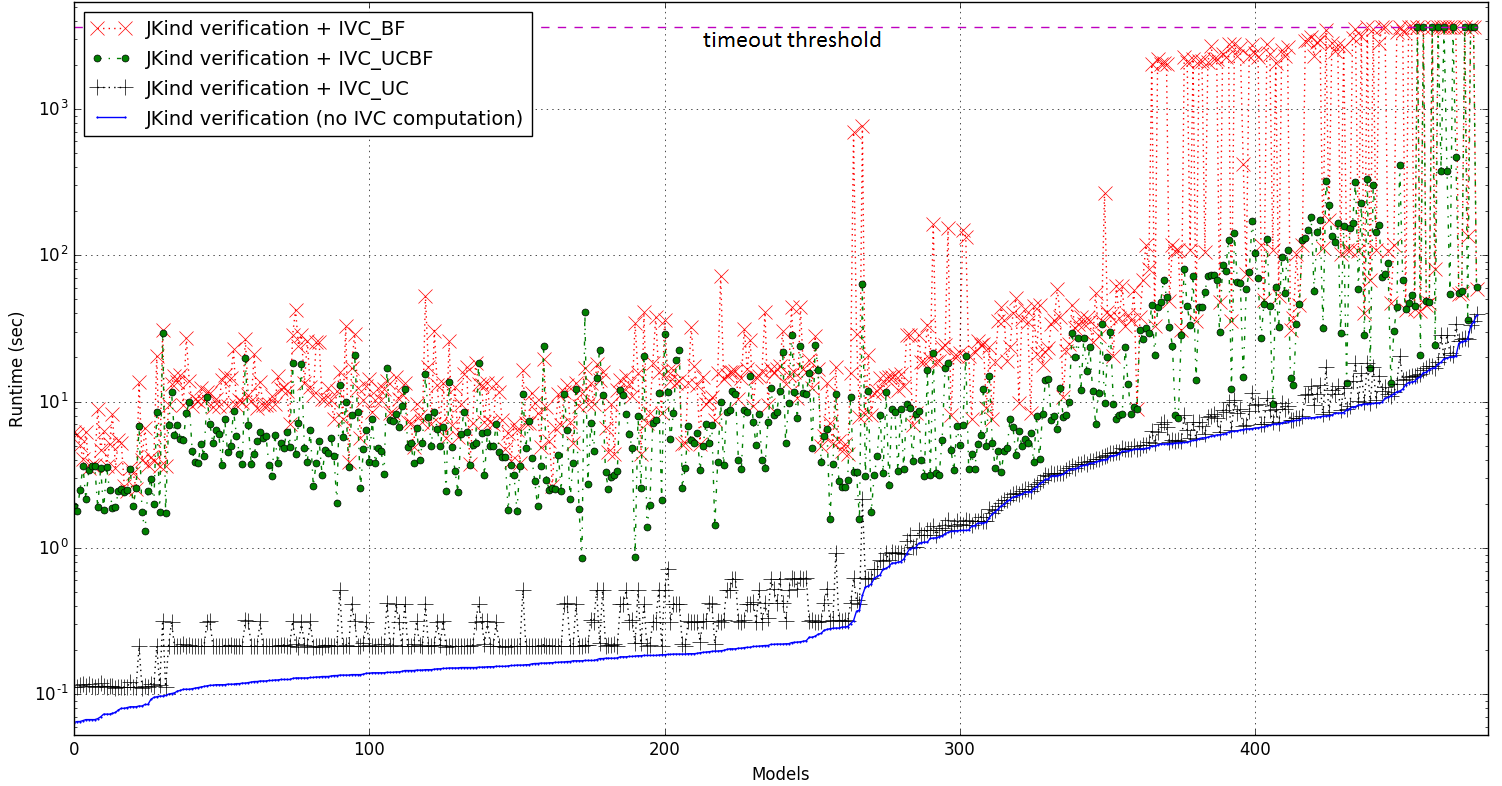
\includegraphics[width=\textwidth]{figs/timing_analyses.png}
  \vspace{-0.3in}
  \caption{Runtime of \bfalg, \ucbfalg, \ucalg algorithms for Yices}\label{fig:runtimeall}
\end{figure*}

%\vspace{-0.5in}
\begin{figure*}
  \centering
  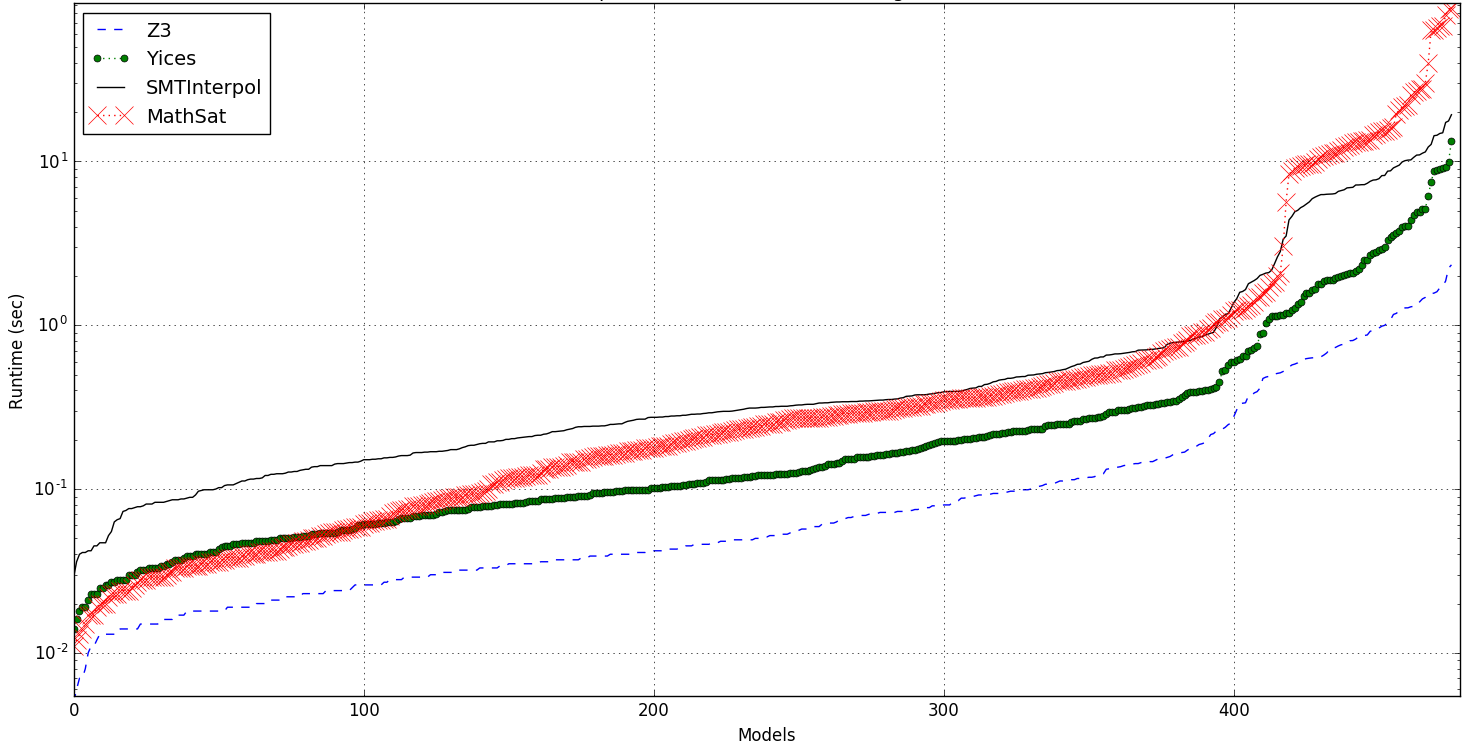
\includegraphics[width=\textwidth]{figs/performance.png}
  \vspace{-0.3in}
  \caption{\ucalg performance on different solvers}\label{fig:performance}
\end{figure*}

\begin{table}
  \centering
  \begin{tabular}{ |c||c|c|c|c| }
    \hline
     runtime (sec) & min & max & mean & stdev \\[0.5ex]
    \hline\hline
 %   JSupport & 2.381 & 165.157 & 21.533 & 23.533 \\[0.5ex]
    Z3   & 0.005 & 2.335 & 0.192 & 0.355 \\[0.5ex]
    Yices &   0.014  & 13.297   & 0.589 & 1.473 \\[0.5ex]
    SMTInterpol& 0.029 & 19.254 &  1.396 & 2.991 \\[0.5ex]
    MathSAT & 0.011 & 86.421 &  3.071 & 10.403 \\[0.5ex]
    \hline
  \end{tabular} \\
  \caption{\ucalg runtime with different solvers}
  \label{tab:runtime-ucalg}
\end{table}

\begin{table}
  \centering
  \begin{tabular}{ |c||c|c|c|c| }
    \hline
     solver & min & max & mean & stdev \\[0.5ex]
    \hline
    Z3   & 0.73\% & 84.13\% & 17.38\% & 16.92\% \\[0.5ex]
    Yices &   0.17\%  & 351.47\%   & 52.20\% & 54.50\% \\[0.5ex]
    SMTInterpol& 1.46\% & 175.75\% &  46.81\% & 37.35\%\\[0.5ex]
    MathSAT & 0.78\% & 955.52\% &  80.21\% & 112.92\%\\[0.5ex]
    \hline
  \end{tabular}
  \caption{Overhead of \ucalg computations using different solvers}
  \label{tab:overhead-ucalg}
\end{table}

\begin{table}
  \centering
  \begin{tabular}{ |c||c|c|c|c| }
    \hline
     runtime (sec) & min & max & mean & stdev \\[0.5ex]
    \hline
    Yices &   0.678  & 3600.0   & 91.594 & 490.008 \\[0.5ex]
    \hline
  \end{tabular}
  \caption{\ucbfalg runtime with Yices}
  \label{tab:runtime-ucbfalg}
\end{table}

\begin{table}
  \centering
  \begin{tabular}{ |c||c|c|c|c| }
    \hline
     solver & min & max & mean & stdev \\[0.5ex]
    \hline
    Yices & 122.50\%  & 30092.78\%   & 3195.90\% & 3896.05\% \\[0.5ex]
    \hline
  \end{tabular}
  \caption{Overhead of \ucbfalg algorithm using Yices}
  \label{tab:overhead-ucbfalg}
\end{table}
% over = in

\begin{table}
  \centering
  \begin{tabular}{ |c|c|c|c| }
    \hline
     solver & PDR & k-induction & \textbf{total} \\
    \hline
      z3 & 2378 & 2379 & 4757 \\
      yices & 2384 & 2376 & 4760 \\
      MathSAT & 2375 & 2369 & 4744 \\
      SMTInterpol & 2378 & 2368 & 4746 \\
    \hline
      \textbf{total} & 9515 & 9492 &   \\
    \hline
  \end{tabular}
  \caption{Aggregate IVC sizes produced by \ucalg\ using different inductive algorithms and solvers}
  \label{tab:minimality-algorithm-solvers}
\end{table}

\begin{table}
  \centering
  \begin{tabular}{ |c||c|c|c|c| }
    \hline
     solver & min & max & mean & stdev \\[0.5ex]
    \hline
    Yices &   0.0\%   & 7.25\% & 0.20\% & 0.50\% \\[0.5ex]
    \hline
  \end{tabular}
  \caption{Increase in IVC Size for \ucalg\ vs. \ucbfalg}
  \label{tab:overhead-ucbfalg}
\end{table}


\begin{figure*}
  \centering
  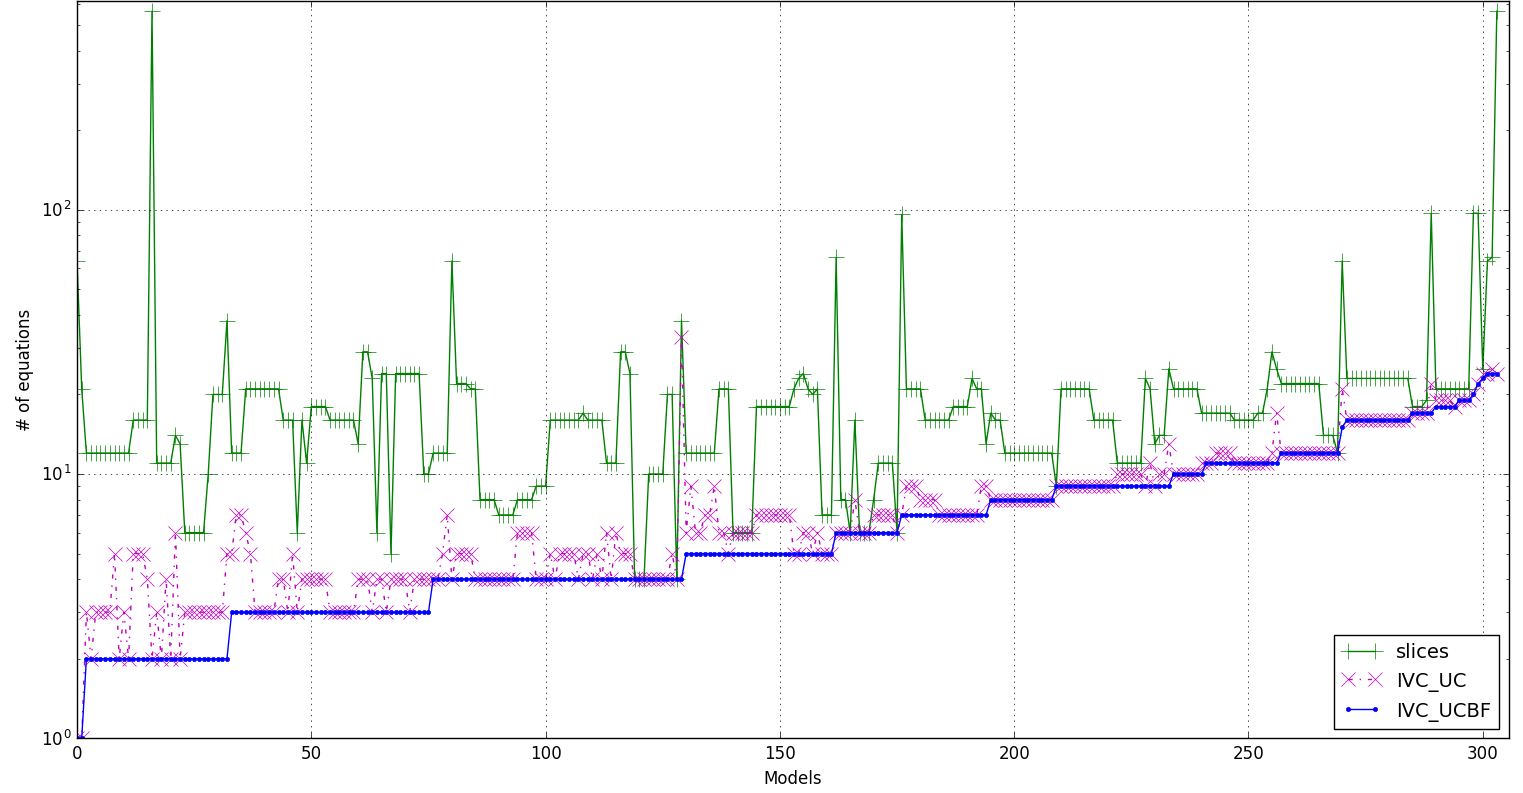
\includegraphics[width=\textwidth]{figs/minimality.png} 
  \caption{IVC sizes produced by \ucalg vs. \ucbfalg for Yices}
  \label{fig:minimality-all}
\end{figure*}

\subsection{Minimality}
\label{sec:minimality}
In this section, we examine the minimality of the cores computed by the \ucalg algorithm using different inductive proof methods and compare it to the cores produced by the combined algorithm (\textbf{RQ2}).  There are three interesting aspects to be examined related to this research question.  First (\textbf{RQ2.1}), does the choice of SMT solver or algorithm used to produce a proof (k-induction or PDR) matter in terms of the minimality of the inductive core?   As mentioned in Section~\ref{sec:ivc}, the \ucalg algorithm is not guaranteed to produce a minimal core due in part to the role of invariants used in producing a proof; as k-induction and PDR use different invariant generation algorithms, it is possible that one or the other is more likely to yield smaller invariant sets.  In addition, differences in the choice of the UNSAT-core algorithms in the different tools could affect the size of the generated core.  However, our algorithm {\em already} does a minimization step.  However,
our algorithm {\em already} does a minimization step on UNSAT-cores,
thus the only differences would be due to one algorithm leading to a
different minimal core than another.

As discussed in Section~\ref{sec:experiment}, k-induction is unable to solve all of the analysis problems; therefore we include only models that are solvable using {\em both} k-induction and PDR by {\em all tools}, 304 models in all.  Examining the aggregate data in Table~\ref{tab:minimality-algorithm-solvers}, we can see the sizes of cores produced by different algorithms and tools.

%if we sum all elements of all cores together, that PDR has an smaller core size in aggregate than k-induction.
%However, the data is noisy, and to examine \textbf{RQ2.1} systematically, we construct a hypothesis that PDR will, in general, equal or outperform k-induction on an arbitrary model:

%\mike{ADD HYPOTHESIS/NULL HYPOTHESIS HERE}

%Although the aggregate data suggests that PDR will yield a smaller core (on average) than k-induction, this claim is not supported for a given model with significance.

\takeaway{Neither PDR nor k-induction yields a smaller inductive validity core in general.}


%we already perform a linear scan of the cores generated by the SMT solver to remove unnecessary conjuncts

The next question (\textbf{RQ2.2}) asks how close to minimal are the cores produced by \ucalg\ vs. the (guaranteed minimal) cores produced by the \ucbfalg\ algorithm?  Note that we cannot measure the distance on all models because the combined algorithm times out on 9 of the larger models.  We therefore examine the distance from minimal cores produced by the combined algorithm for models in which it completes within the one hour timeout.  For comparison, we run the \ucalg\ algorithm in each tool with the default {\em fastest} algorithm, which will use the result of either k-induction or PDR.  A graph showing the size of the IVCs for each model produced by the yices solver is shown in Figure~\ref{fig:minimality-all}.  In the figure, the models are ranked along the x-axis by the size of the core produced by \ucbfalg.  The figure demonstrates that while on average there is a modest change in minimality that there can be substantial variance on the sizes of the cores produced by the \ucalg\ algorithm.

\takeaway{The \ucalg algorithm computes cores that are 0\% to 7.25\% larger than those produced by \ucbfalg, with substantial variance in the results.}


\iffalse
\ela{I think this is not needed: \\In terms of size, we calculated the size of the biggest and smallest sets per model, then added them together for all models. The same calculation has been done for \texttt{JSupport}:
\begin{itemize}
  \item $A\_JS$: the aggregate number of elements in support sets computed by \texttt{JSupport} = 3078
  \item $A\_Ss$: the aggregate number of elements in the \emph{smallest} support sets = 3474;
  this implies $A\_Ss$ is 12\% greater than $A\_JS$.
  \item $A\_Bs$: the aggregate number of elements in the \emph{biggest} support sets = 3586;
  this implies $A\_Bs$ is 16\% greater than $A\_JS$.
\end{itemize}}
Average size of sets computed by \texttt{ReduceSupport} is 8.55. And, average size of sets computed by \texttt{JSupport} is 7.60. Therefore, in average, support sets computed by \texttt{ReduceSupport} are 88\% close to minimal, in terms of their size.  %  (1 - ((8.55 - 7.6)/ 7.6))  * 100 = 87.5%
Since \texttt{JSupport}, with a great percentage, most of the time computed the smallest support set, we compared the size of the sets computed by \texttt{ReduceSupport} with \texttt{JSupport}. For each configuration, we collected the difference between its support size and \texttt{JSupport} per model. Table~\ref{tab:minimality} shows the result of analysis.
\fi

\begin{table}
  \centering
  \begin{tabular}{ |c|c|c|c| }
    \hline
     min & max & mean & stdev \\[0.5ex]
    \hline
    %sample size = 4196
     0.0   & 0.878 & 0.026 & 0.059 \\[0.5ex]
    \hline
  \end{tabular}
  \caption{Pairwise Jaccard distances among all models}
  \label{tab:jaccard-avg}
\end{table}

\begin{figure*}
  \centering
  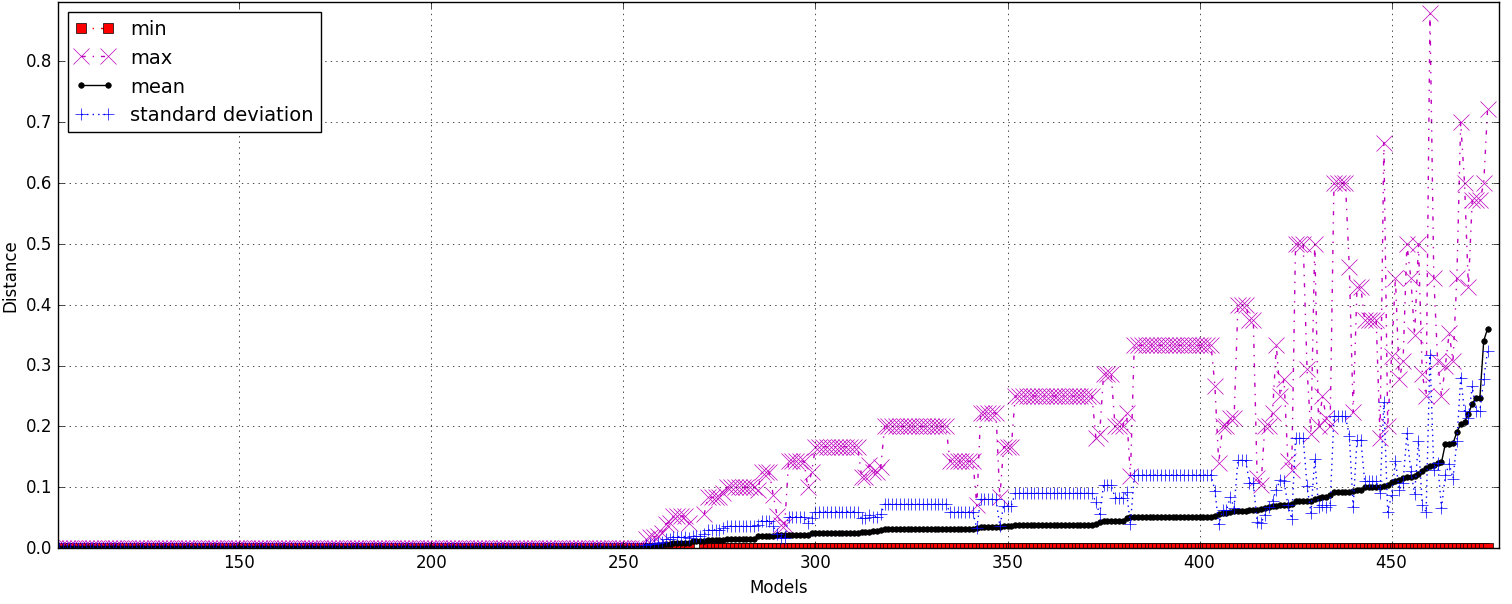
\includegraphics[width=\textwidth]{figs/jacdis2.png} \\
  \caption{Pairwise Jaccard distance between IVCs}\label{fig:jacdis}
\end{figure*}

\subsection{Diversity}
\label{sec:diversity}
Recall from Section~\ref{sec:ivc} that a {\em minimal} core is any core leading to a proof such that if you remove any of the conjuncts from the core, it no longer produces a proof.  For certain models and properties, it is possible that there are many minimal cores that will lead to a proof.  In this section, we examine the issue of diversity: do different tools and algorithms lead to {\em different} minimal cores?  This is both a function of the models and the solution algorithms: for certain models, there is only one possible minimal core, whereas other models might have many. Given that there are multiple solutions, the interesting question is whether using different tools and algorithms will lead to different solutions.  Note that this question is closely tied to that of {\em minimality}, which we examined in the previous section.

Our exploration in this case is not exhaustive, but only exploratory.  The reason it is considered is that it has substantial relevance to some of the uses of the tool: e.g., for constructing traceability matrices from proofs.  Given diversity of results, we may wish to distinguish {\em must} traceability elements from {\em may} traceability elements across a set of diverse solutions, and consider more systematic explorations of diversity in future work.

To measure diversity of IVCs, we use Jaccard distance:
\begin{definition}{\emph{Jaccard distance:}}
  \label{def:dj}
  $d_J(\small{A}, \small{B}) = 1 - \frac{|A \cap B|}{|A \cup B|} ,\\ 0 \leq d_J(\small{A}, \small{B}) \leq 1$
\end{definition}
\noindent Jaccard distance is a standard metric for comparing finite sets (assuming that both sets are non-empty) by comparing the size of the intersection of two sets over its union.  For each model in the benchmark, the experiments generated 13 different sets of support. Therefore, we obtained $\binom{13}{2} = 78$ combinations of pairwise distances per model. Then, minimum, maximum, average, and standard deviation of the distances were calculated (Fig~\ref{fig:jacdis}), by which, again, we calculated these four measures among all models.  As seen in Table~\ref{tab:jaccard-avg}, on average, the Jaccard distance between different solutions is small, but the maximum is close to 1, which indicates that even for our exploratory analysis, there are models for which the tools yield substantially diverse solutions.  The diversity between solutions is represented graphically in Figure~\ref{fig:jacdis}, where for each model, we present the min, max, and mean pairwise distance of the solutions produced by algorithm \ucalg for each model, ranked by the mean distance.

\iffalse
\mike{Do we want the discussion below?  I am not sure that it adds much}

To measure the overall similarity among all sets, instead of a pairwise comparison, we used \emph{frequent pattern mining} \cite{han2007frequent}. To define an overall similarity among all sets of support of a given model\footnote{Note that all models in the benchmarks are single property; hence, instead of saying a set of support of a given \emph{property}, we just refer it as the support set of the \emph{model} while explaining the experimental results.}, we calculated a \emph{core} support set for each model in the benchmark, which can be considered as a closed frequent pattern; a core set of model $M$, denoted by $C_M$, is defined as:
\begin{definition}
  \label{def:core}
  $C_M = \bigcap_{i=1}^{13} s_{Mi},   \hspace{9pt} s_{Mi} \in S_M$
\end{definition}

Based on this notion, overall dissimilarity, denoted by $D_{J\{M\}}$, is defined as follows:

\begin{definition}
  \label{def:dis}
  $D_{J\{M\}} =  \frac{\sum_{i=1}^{12}d_J(s_{Mi}, C_M)}{12},   \hspace{9pt} s_{Mi} \in S_M$
\end{definition}

Since our goal is to measure the diversity or dissimilarity among sets computed by \texttt{ReduceSupport}, in \ref{def:dis}, we exclude the set generated by \texttt{JSupport}. In Fig~\ref{fig:jacdis}, the \emph{overall distance} line shows $D_{J\{M\}}$ per model, which can be analyzed from the following hypotheses:
\begin{itemize}
  \item H0: variety of obtained sets of support is high (average $D_{J\{M\}}$ of 0.2)
  \item H1: variety of obtained sets of support is small (average $D_{J\{M\}}$ less than 0.2)
\end{itemize}
Table~\ref{tab:variety} shows that, with an effect size of 0.79, H0 can be rejected.
\begin{table}
  \centering
  \begin{tabular}{ |c|c|c|c|c|c| }
    \hline
     min & max & mean & stdev & ES & p-value\\[0.5ex]
    \hline
    %sample size = 395
     0.0   & 0.879 & 0.099 & 0.141 & 0.72 & < 0.00001 \\[0.5ex]
    \hline
  \end{tabular}
  \caption{$D_{J\{M\}}$ among all models}
  \label{tab:variety}
\end{table}
\fi
%summarized as follows:
%\begin{itemize}
%  \item minimum $D_{J\{M\}}$ among all models: 0.0
%  \item maximum $D_{J\{M\}}$ among all models: 0.879
%  \item average $D_{J\{M\}}$ among all models: 0.096
%  \item standard deviation of $D_{J\{M\}}$ among all models: 0.132
%\end{itemize}


\subsection{Discussion}

In the previous section, we presented three algorithms for determining inductive validity cores.  The brute-force algorithm is guaranteed minimal, but is often very slow.  The other two algorithms: the UNSAT-core algorithm \ucalg\ and the combined algorithm \ucbfalg, represent interesting trade-offs.  The \ucalg\ algorithm is much faster, but is not guaranteed to be minimal; the result of this algorithm can be further, and often quite quickly, refined by the combined algorithm.  Thus, we can choose to trade off speed for guaranteed minimality using these two algorithms; the combined algorithm can be viewed as a refinement algorithm that we can terminate either at completion or after a fixed time bound.


%One question that arises is: why is the refinement so much quicker than the brute-force approach?  In our preliminary examination, it appears to be because of the actions performed by JKind on the sub-problems.  When the cores produced by \ucalg\ are minimal or close to minimal, it tends to be the case that removing conjuncts from the core leads to short counterexamples.  When performing the brute-force algorithm, removing the irrelevant pieces of the model require repeated proof search.

Although our experiment does not ask statistical questions, it is still worth examining threats towards generalizing our results.  First, are the models and properties that we chose representative?  We started from an existing benchmark from another research group suite to try to assuage this concern, but most of these models were small, so we extended the benchmark suite with 81 of our own models.  It is possible that our additions skew the results, though these models are immediately derived from previously published work and not modified for our analysis here.  Second, our models and tools use the Lustre language, which is equational, rather than conjuncted transition systems; it is possible (though, in our opinion, unlikely) that arbitrary conjuncts rather than equations will yield different performance or minimality characteristics.

 